\documentclass{beamer}

% xcolor and define colors -------------------------
\usepackage{xcolor}

% https://www.viget.com/articles/color-contrast/
\definecolor{purple}{HTML}{5601A4}
\definecolor{navy}{HTML}{0D3D56}
\definecolor{ruby}{HTML}{9a2515}
\definecolor{alice}{HTML}{107895}
\definecolor{daisy}{HTML}{EBC944}
\definecolor{coral}{HTML}{F26D21}
\definecolor{kelly}{HTML}{829356}
\definecolor{cranberry}{HTML}{E64173}
\definecolor{jet}{HTML}{131516}
\definecolor{asher}{HTML}{555F61}
\definecolor{slate}{HTML}{314F4F}

% Mixtape Sessions
\definecolor{picton-blue}{HTML}{00b7ff}
\definecolor{violet-red}{HTML}{ff3881}
\definecolor{sun}{HTML}{ffaf18}
\definecolor{electric-violet}{HTML}{871EFF}

\newcommand\pictonBlue[1]{{\color{picton-blue}#1}}
\newcommand\sun[1]{{\color{sun}#1}}
\newcommand\electricViolet[1]{{\color{electric-violet}#1}}
\newcommand\violetRed[1]{{\color{violet-red}#1}}

\newcommand\bgPictonBlue[1]{{\colorbox{picton-blue!20!white}{#1}}}
\newcommand\bgSun[1]{{\colorbox{sun!20!white}{#1}}}
\newcommand\bgElectricViolet[1]{{\colorbox{electric-violet!20!white}{#1}}}
\newcommand\bgVioletRed[1]{{\colorbox{violet-red!20!white}{#1}}}

\def\code#1{\texttt{#1}}

% Main theme colors
\definecolor{accent}{HTML}{00b7ff}
\definecolor{accent2}{HTML}{871EFF}
\definecolor{gray100}{HTML}{f3f4f6}
\definecolor{gray800}{HTML}{1F292D}


% Beamer Options -------------------------------------

% Background
\setbeamercolor{background canvas}{bg = white}

% Change text margins
\setbeamersize{text margin left = 15pt, text margin right = 15pt} 

% \alert
\setbeamercolor{alerted text}{fg = accent2}

% Frame title
\setbeamercolor{frametitle}{bg = white, fg = jet}
\setbeamercolor{framesubtitle}{bg = white, fg = accent}
\setbeamerfont{framesubtitle}{size = \small, shape = \itshape}

% Block
\setbeamercolor{block title}{fg = white, bg = accent2}
\setbeamercolor{block body}{fg = gray800, bg = gray100}

% Title page
\setbeamercolor{title}{fg = gray800}
\setbeamercolor{subtitle}{fg = accent}

%% Custom \maketitle and \titlepage
\setbeamertemplate{title page}
{
    %\begin{centering}
        \vspace{20mm}
        {\Large \usebeamerfont{title}\usebeamercolor[fg]{title}\inserttitle}\\
        {\large \itshape \usebeamerfont{subtitle}\usebeamercolor[fg]{subtitle}\insertsubtitle}\\ \vspace{10mm}
        {\insertauthor}\\
        {\color{asher}\small{\insertdate}}\\
    %\end{centering}
}

% Table of Contents
\setbeamercolor{section in toc}{fg = accent!70!jet}
\setbeamercolor{subsection in toc}{fg = jet}

% Button 
\setbeamercolor{button}{bg = accent}

% Remove navigation symbols
\setbeamertemplate{navigation symbols}{}

% Table and Figure captions
\setbeamercolor{caption}{fg=jet!70!white}
\setbeamercolor{caption name}{fg=jet}
\setbeamerfont{caption name}{shape = \itshape}

% Bullet points

%% Fix spacing between items
\let\olditemize=\itemize 
\let\endolditemize=\enditemize 
\renewenvironment{itemize}{\vspace{0.25em}\olditemize \itemsep0.25em}{\endolditemize}

%% Fix left-margins
\settowidth{\leftmargini}{\usebeamertemplate{itemize item}}
\addtolength{\leftmargini}{\labelsep}

%% enumerate item color
\setbeamercolor{enumerate item}{fg = accent}
\setbeamerfont{enumerate item}{size = \small}
\setbeamertemplate{enumerate item}{\insertenumlabel.}

%% itemize
\setbeamercolor{itemize item}{fg = accent!70!white}
\setbeamerfont{itemize item}{size = \small}
\setbeamertemplate{itemize item}[circle]

%% right arrow for subitems
\setbeamercolor{itemize subitem}{fg = accent!60!white}
\setbeamerfont{itemize subitem}{size = \small}
\setbeamertemplate{itemize subitem}{$\rightarrow$}

\setbeamertemplate{itemize subsubitem}[square]
\setbeamercolor{itemize subsubitem}{fg = jet}
\setbeamerfont{itemize subsubitem}{size = \small}








% Links ----------------------------------------------

\usepackage{hyperref}
\hypersetup{
  colorlinks = true,
  linkcolor = accent2,
  filecolor = accent2,
  urlcolor = accent2,
  citecolor = accent2,
}


% Line spacing --------------------------------------
\usepackage{setspace}
\setstretch{1.35}


% \begin{columns} -----------------------------------
\usepackage{multicol}


% Fonts ---------------------------------------------
% Beamer Option to use custom fonts
\usefonttheme{professionalfonts}

% \usepackage[utopia, smallerops, varg]{newtxmath}
% \usepackage{utopia}
\usepackage[sfdefault,light]{roboto}

% Small adjustments to text kerning
\usepackage{microtype}



% Remove annoying over-full box warnings -----------
\vfuzz2pt 
\hfuzz2pt


% Table of Contents with Sections
\setbeamerfont{myTOC}{series=\bfseries, size=\Large}
\AtBeginSection[]{
        \frame{
            \frametitle{Roadmap}
            \tableofcontents[current]   
        }
    }


% Tables -------------------------------------------
% Tables too big
% \begin{adjustbox}{width = 1.2\textwidth, center}
\usepackage{adjustbox}
\usepackage{array}
\usepackage{threeparttable, booktabs, adjustbox}
    
% Fix \input with tables
% \input fails when \\ is at end of external .tex file
\makeatletter
\let\input\@@input
\makeatother

% Tables too narrow
% \begin{tabularx}{\linewidth}{cols}
% col-types: X - center, L - left, R -right
% Relative scale: >{\hsize=.8\hsize}X/L/R
\usepackage{tabularx}
\newcolumntype{L}{>{\raggedright\arraybackslash}X}
\newcolumntype{R}{>{\raggedleft\arraybackslash}X}
\newcolumntype{C}{>{\centering\arraybackslash}X}

% Figures

% \imageframe{img_name} -----------------------------
% from https://github.com/mattjetwell/cousteau
\newcommand{\imageframe}[1]{%
    \begin{frame}[plain]
        \begin{tikzpicture}[remember picture, overlay]
            \node[at = (current page.center), xshift = 0cm] (cover) {%
                \includegraphics[keepaspectratio, width=\paperwidth, height=\paperheight]{#1}
            };
        \end{tikzpicture}
    \end{frame}%
}

% subfigures
\usepackage{subfigure}


% Highlight slide -----------------------------------
% \begin{transitionframe} Text \end{transitionframe}
% from paulgp's beamer tips
\newenvironment{transitionframe}{
    \setbeamercolor{background canvas}{bg=accent!40!black}
    \begin{frame}\color{accent!10!white}\LARGE\centering
}{
    \end{frame}
}


% Table Highlighting --------------------------------
% Create top-left and bottom-right markets in tabular cells with a unique matching id and these commands will outline those cells
\usepackage[beamer,customcolors]{hf-tikz}
\usetikzlibrary{calc}
\usetikzlibrary{fit,shapes.misc}

% To set the hypothesis highlighting boxes red.
\newcommand\marktopleft[1]{%
    \tikz[overlay,remember picture] 
        \node (marker-#1-a) at (0,1.5ex) {};%
}
\newcommand\markbottomright[1]{%
    \tikz[overlay,remember picture] 
        \node (marker-#1-b) at (0,0) {};%
    \tikz[accent!80!jet, ultra thick, overlay, remember picture, inner sep=4pt]
        \node[draw, rectangle, fit=(marker-#1-a.center) (marker-#1-b.center)] {};%
}


% DAGS ----------------------------------------------
\usepackage{tikz}
\usetikzlibrary{shapes,decorations,arrows,calc,arrows.meta,fit,positioning}
% Tikz settings optimized for causal graphs.
\tikzset{
    -Latex,auto,node distance =1 cm and 1 cm,semithick,
    state/.style ={ellipse, draw, minimum width = 0.7 cm},
    point/.style = {circle, draw, inner sep=0.04cm,fill,node contents={}},
    bidirected/.style={Latex-Latex,dashed},
    el/.style = {inner sep=2pt, align=left, sloped}
}


% Beamer tricks -------------------------------------
% Make \pause work in align environments
\makeatletter
\renewrobustcmd{\beamer@@pause}[1][]{%
  \unless\ifmeasuring@%
  \ifblank{#1}%
    {\stepcounter{beamerpauses}}%
    {\setcounter{beamerpauses}{#1}}%
  \onslide<\value{beamerpauses}->\relax%
  \fi%
}
\makeatother

\usepackage{breqn} % Breaks lines

\usepackage{amsmath}
\usepackage{mathtools}

\usepackage{pdfpages} % \includepdf

\usepackage{listings} % R code
\usepackage{verbatim} % verbatim

% Video stuff
\usepackage{media9}

% packages for bibs and cites
\usepackage{natbib}
\usepackage{har2nat}
\newcommand{\possessivecite}[1]{\citeauthor{#1}'s \citeyearpar{#1}}
\usepackage{breakcites}
\usepackage{alltt}

% Setup math operators
\DeclareMathOperator{\E}{E} \DeclareMathOperator{\tr}{tr} \DeclareMathOperator{\se}{se} \DeclareMathOperator{\I}{I} \DeclareMathOperator{\sign}{sign} \DeclareMathOperator{\supp}{supp} \DeclareMathOperator{\plim}{plim}
\DeclareMathOperator*{\dlim}{\mathnormal{d}\mkern2mu-lim}
\newcommand\independent{\protect\mathpalette{\protect\independenT}{\perp}}
   \def\independenT#1#2{\mathrel{\rlap{$#1#2$}\mkern2mu{#1#2}}}
\newcommand*\colvec[1]{\begin{pmatrix}#1\end{pmatrix}}

\newcommand{\myurlshort}[2]{\href{#1}{\textcolor{gray}{\textsf{#2}}}}


\begin{document}

\imageframe{./lecture_includes/mixtape_did_cover.png}


% ---- Content ----

\section{Stacking}

\subsection{Motivating example: Minimum wages}


\begin{frame}{Keep TWFE but avoid differential timing problems}

\begin{itemize}
\item Problem with the canonical TWFE specification was the explicit use of already-treated as controls introduced biases
\item CS and SA estimated each feasible group-time ATT (``cohort-specific ATT'') then summarized into a reasonably weighted ATT
\item Differences between the two had to do with incorporating covariates and who was chosen as controls (CS and SA used the never-treated (CS and SA), not-yet-treated (CS) or last-treated (SA) as controls)
\item Could we still use TWFE, but avoid the use of already-treated as controls?  How? Interpretation?
\end{itemize}

\end{frame}


\begin{frame}{Stacking minimum wages}

\begin{itemize}
\item  Cengiz, et al. (2019) call this ``clean controls'' but now it's called ``stacking'' (Baker, et al. 2022)
\item Very good example (like Miller, et al. 2021) for how to build an argument through tables, figures and various forms of intuitive reasoning that guides estimation
\item Data is 1979 to 2016 US state-level panel, 138 ``prominent'' state-level minimum wage change events
\item Main model specification is TWFE, but in a robustness section (Appendix D) they introduce the ``stacking'' alternative
\end{itemize}

\end{frame}

\begin{frame}{Background}

\begin{itemize}
\item Theory is ambiguous with respect to increasing minimum binding minimum wages on employment/unemployment 
	\begin{itemize}
	\item On the one hand, minimum wages should reduce employment in \textbf{perfectly competitive labor markets}. Minimize cost subject to isoquant constraint, solve for first order conditions, $\frac{d L*(w,r,q)}{d w<0}$. No Giffen behavior with labor inputs.
	\item But, minimum wages will increase employment in \textbf{imperfect labor markets}. See Joan Robinson's monopsony work 
	\end{itemize}
\item Early work on this was viewed as low quality but gradually improved; back-and-forth debates have tended to leave the questions temporarily settled before being overturned
\end{itemize}
\end{frame}

\begin{frame}{Background}

\begin{itemize}
\item Prior research: ``new minimum wage'' studies starting with the now classic Card and Krueger (1994) which found no effect of minimum wages on employment, but others (many written by David Neumark) found reductions in employment
\item Prior research had often been on \textbf{aggregate} employment or teenagers
\item This paper will use less aggregated data but in an unusual way I hadn't seen before
\end{itemize}

\end{frame}

\begin{frame}{Data}

\begin{quote}
``We use the individual-level NBER Merged Outgoing Rotation Group of the CPS for 1979-2016 to calculate quarterly, state-level distributions of hourly wages. For hourly workers, we use the reported hourly wage, and for other workers, we define the hourly wage to be their usual weekly earnings divided by usual weekly hours.  We do not use any observations with imputed wage data to minimize the role of measurement error.''
\end{quote}


\end{frame}

\begin{frame}{Data}

\begin{itemize}
\item Hourly wage data from 1976-2016 NBER out-rotation group of the Current Population Survey broken into wage bins (by \$0.25) from \$0 to \$30
\item Wages are deflated to 2016 dollars to get ``real wage''
\item There are 117 wage bins that are then collapsed into quarterly, state-level employment counts $E_{swt}$ using person-level sampling weights
\item Why are they doing this? What's wrong with just regressing state-level employment onto minimum hikes?
\end{itemize}

\end{frame}

\begin{frame}{Minimum wage data}

\begin{itemize}
\item They get their minimum wage data from Vaghul and Zipperer (2016) which shows quarterly max of the state-level daily minimum wage series 
\item Paper focuses on 138 treatments or minimum wage events, of which 8.6\% of workers were below the minimum wage the year before the event
\item Focus is inductive reasoning -- concepts are ``missing'' vs ``excess'' jobs equal to different treatment effects in employment by wage bins just above and just below the minimum wage cutoff
\end{itemize}

\end{frame}

\begin{frame}{Remember my philosophy on DiD}

\begin{enumerate}
\item[1. ] \textbf{Show bite}. People \emph{need} to see first order effects and they need to be large.  
	\begin{itemize}
	\item Oftentimes we focus only secondary effects -- sex work legalization effect on STIs or violence (Cunningham and Shah 2018) 
	\item Economics loves counter intuitive results, and they dominate our attention, but they're not credible if we can't show bite oftentimes
	\item Bite requires the most creativity of all probably as it's finding data and finding theories
	\end{itemize}
\end{enumerate}

\end{frame}

\begin{frame}{This Paper's Bite}

\begin{quote}
``When we refer to the `bite' of the minimum wage, or to the extent to which the minimum wage is `binding', we mean how effective the minimum wage is in raising wages at the bottom.  Therefore, the bite is a function of (i) how many workers are earning below the minimum wage, (ii) how many of those workers are legally covered by the policy, and (iii) the extent of compliance.''
\end{quote}

\end{frame}



\begin{frame}{Remember my philosophy on DiD}

\begin{enumerate}
\item[2. ] \textbf{Falsifications}. 
	\begin{itemize}
	\item Your main results show effects where you expect them
	\item Your falsifications do not find effects where there should be no effects
	\item This style of reasoning is unique to the applied work outside the RCT;
	\item Less common outside econ (though you did see it John Snow's original cholera studies ironically)
	\item Think carefully -- it must be based on logic and shared opinions
	\end{itemize}
\end{enumerate}

\end{frame}


\begin{frame}{Remember my philosophy on DiD}

\begin{enumerate}
\item[3. ] \textbf{Event studies}. 
	\begin{itemize}
	\item Event studies support basic ideas like having found good controls, no anticipation, plausible parallel trends
	\item The visuals are key -- they support the interpretation of the coefficients as dynamic ATT parameters
	\end{itemize}
\end{enumerate}

\end{frame}




\begin{frame}{Rhetorical argument}

\begin{itemize}
\item Key visual showing excess vs missing jobs helps communicate the idea of ``bite'' which supports all subsequent analysis
\item If no bite, no effects shown can be plausibly causal -- so notice, the logic of identification comes from convincingly showing bite, not from the model results themselves
\item Carefully construct data into bins so that narrowly employment above and below the minimum wage can be measured
\item Do the same for employment per population
\item Calculate net changes in employment both for total (main results) and by various slices (heterogenous effects)
\end{itemize}

\end{frame}

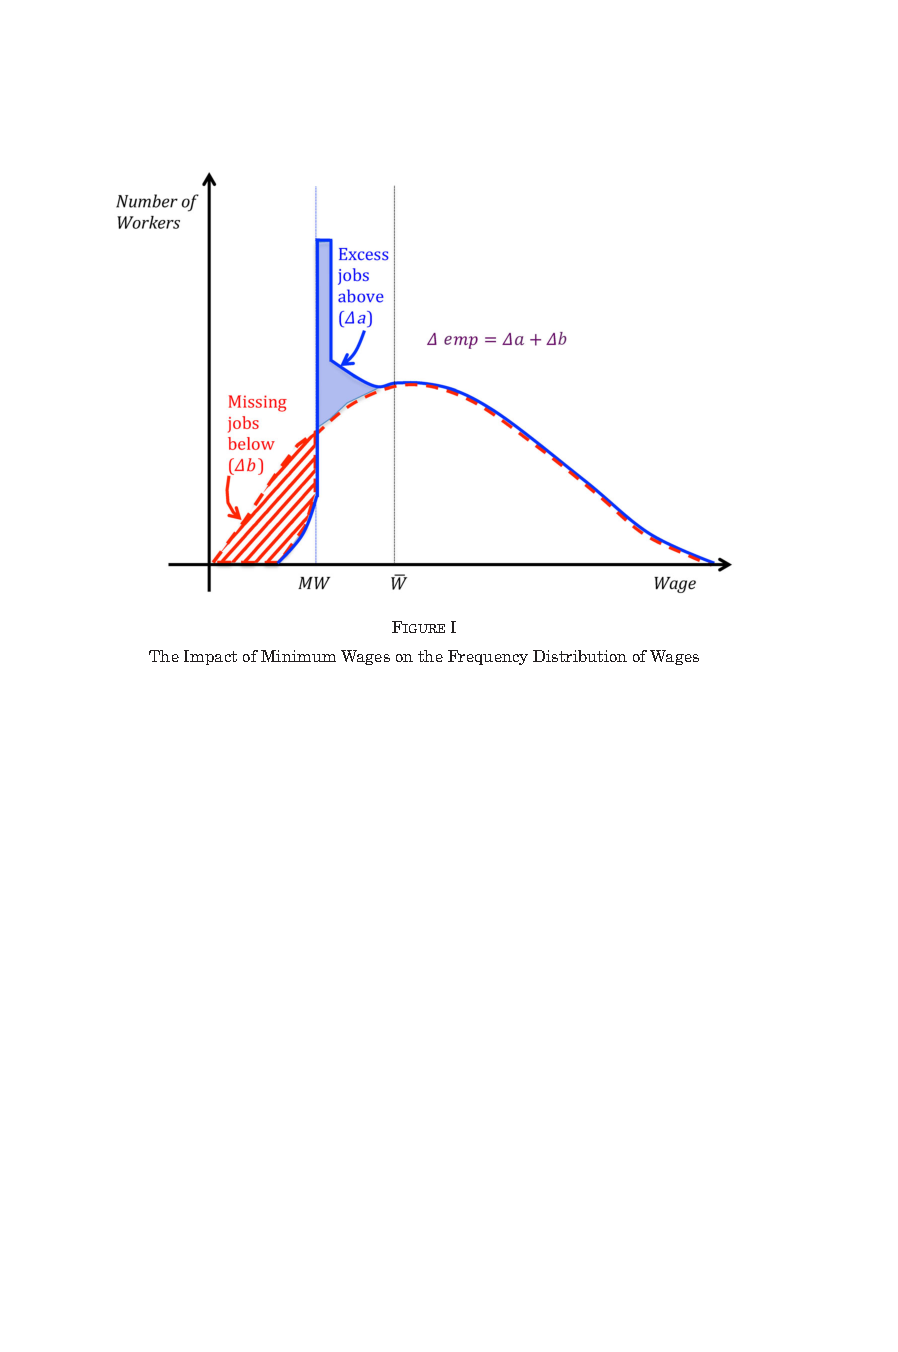
\includegraphics{./lecture_includes/dube_a.pdf}

\begin{frame}{Null results on the event study}

\begin{itemize}
\item Results we will now see is essentially a lot of zeroes (nulls work if they're precise and on a result people may disagree about)
\item Authors fail to find any evidence of an effect on employment other than the ``bite'' result which I'll show
\item Empirical equation is estimated using TWFE; differential timing problems, $\tau$ are event years and $k$ are dollar bins, $\mu$ and $\rho$ are state-by-wage-bin and period-by-wage-bin fixed effects, $\omega$ are controls for small or federal increases
\end{itemize}

\begin{equation}
E/N = \sum_{\tau=-3}^4 \sum_{k=-4}^{17} \alpha_{\tau k}I^{\tau k}_{sjt} + \mu_{sj} + \rho_{jt} + \omega_{sjt} + u_{sjt}
\end{equation}

\end{frame}

\imageframe{./lecture_includes/dube_b.pdf}
\imageframe{./lecture_includes/dube_c.pdf}
\imageframe{./lecture_includes/dube_d.pdf}
\imageframe{./lecture_includes/dube_e.pdf}
\imageframe{./lecture_includes/dube_f.pdf}
\imageframe{./lecture_includes/dube_g.pdf}
\imageframe{./lecture_includes/dube_h.pdf}
\imageframe{./lecture_includes/dube_i.pdf}


\subsection{Creating a stacked model}

\begin{frame}{Stacking alternative}

\begin{itemize}
\item Cengiz, et al. (2019) used TWFE with differential timing, much like had always been done, but they have Cambridge connections and SA was in the air (Dube did a sabbatical at MIT)
\item They knew TWFE estimation was biased if there are differential timing and heterogenous treatment effects by cohort in other words
\item They propose their own alternative which they call ``clean controls'' but which is more commonly called ``stacking'' (Baker, et al. 2022)
\item Estimation models are TWFE; weights were unknown at time of writing (but have since been derived by Gardner 2021)
\end{itemize}

\end{frame}

\begin{frame}{Dataset construction}

Clean controls is done one of two ways:
	\begin{enumerate}
	\item Create 138 datasets, one for each event $h$ where the treatment group is one state and the control are all other states that did not have a minimum wage increase in eight-year panels around event $h$, balanced in calendar time, inference must adjust for heteroskedasticity with only one treatment date (Ferman and Pinto Restat)
	\item ``Stack'' the 138 datasets, re-centering each treatment date such that data is balanced in ``event time'' with 3 periods pre-treatment, 4 years post-treatment, and controls are all untreated units from -3 to +4. Several units will appear more than once).
	\end{enumerate}
\bigskip

\end{frame}



\begin{frame}{Steps to stacked regression}
\begin{enumerate}
    \item[1.]  Create separate ``event by cohort specific'' datasets for each policy cohort (e.g., groups who pass minimum wages in the same year)
        \begin{itemize}
        \item Dataset will consist of the relevant policy cohort \textbf{plus} controls
        \item Data is structured in ``event time'' and will be balanced such that panel length is $h$, perhaps starting point being 3 years prior to treatment and ending point 4 years after or something like that
        \item Each dataset will contain individuals untreated over the $h$ period defined
        \end{itemize}
\end{enumerate}
\end{frame}

\begin{frame}{Steps to stacked regression}
\begin{enumerate}
    \item[2. ] Append each dataset (or what people are now calling ``stacking'') to one another
        \begin{itemize}
        \item This necessarily replicates control observations though as they are in each datasets
        \item Since the same people are often appearing many many times, you will correct for this in the regression model specification
        \end{itemize}
    \item[3. ] Estimate a simple 2x2 model but include ``cohort-by-state'' fixed effects so as to account for the multiple appearances of observations from the never-treated control states
\end{enumerate}
\end{frame}

\begin{frame}{Comments on the approach}

\begin{itemize}
\item Hard part of this is probably just the careful balancing, saving datasets, then appending, but ultimately not difficult -- just double and triple check your work using logic and investigating the datasets (there should be no already treated in any dataset for instance)
\item I wouldn't trust someone else's code on this; write the loops yourself. You're responsible.
\end{itemize}

\end{frame}

\begin{frame}{Comments on the approach}

\begin{itemize}
\item Because the data is now balanced \emph{in event time}, there is \emph{no differential timing}; it is a simple 2x2
\item Recall that the reason TWFE is biased in DiD designs is (1) differential timing and (2) heterogeneity
\item Stacked eliminates (1) making (2) irrelevant
\item But recall the lessons we learned about including time-varying covariates from Sant'Anna and Zhao (2020) -- stacked will suffer from those too
\end{itemize}

\end{frame}



\begin{frame}{Imbalanced in relative time with differential timing}

	\begin{figure}
	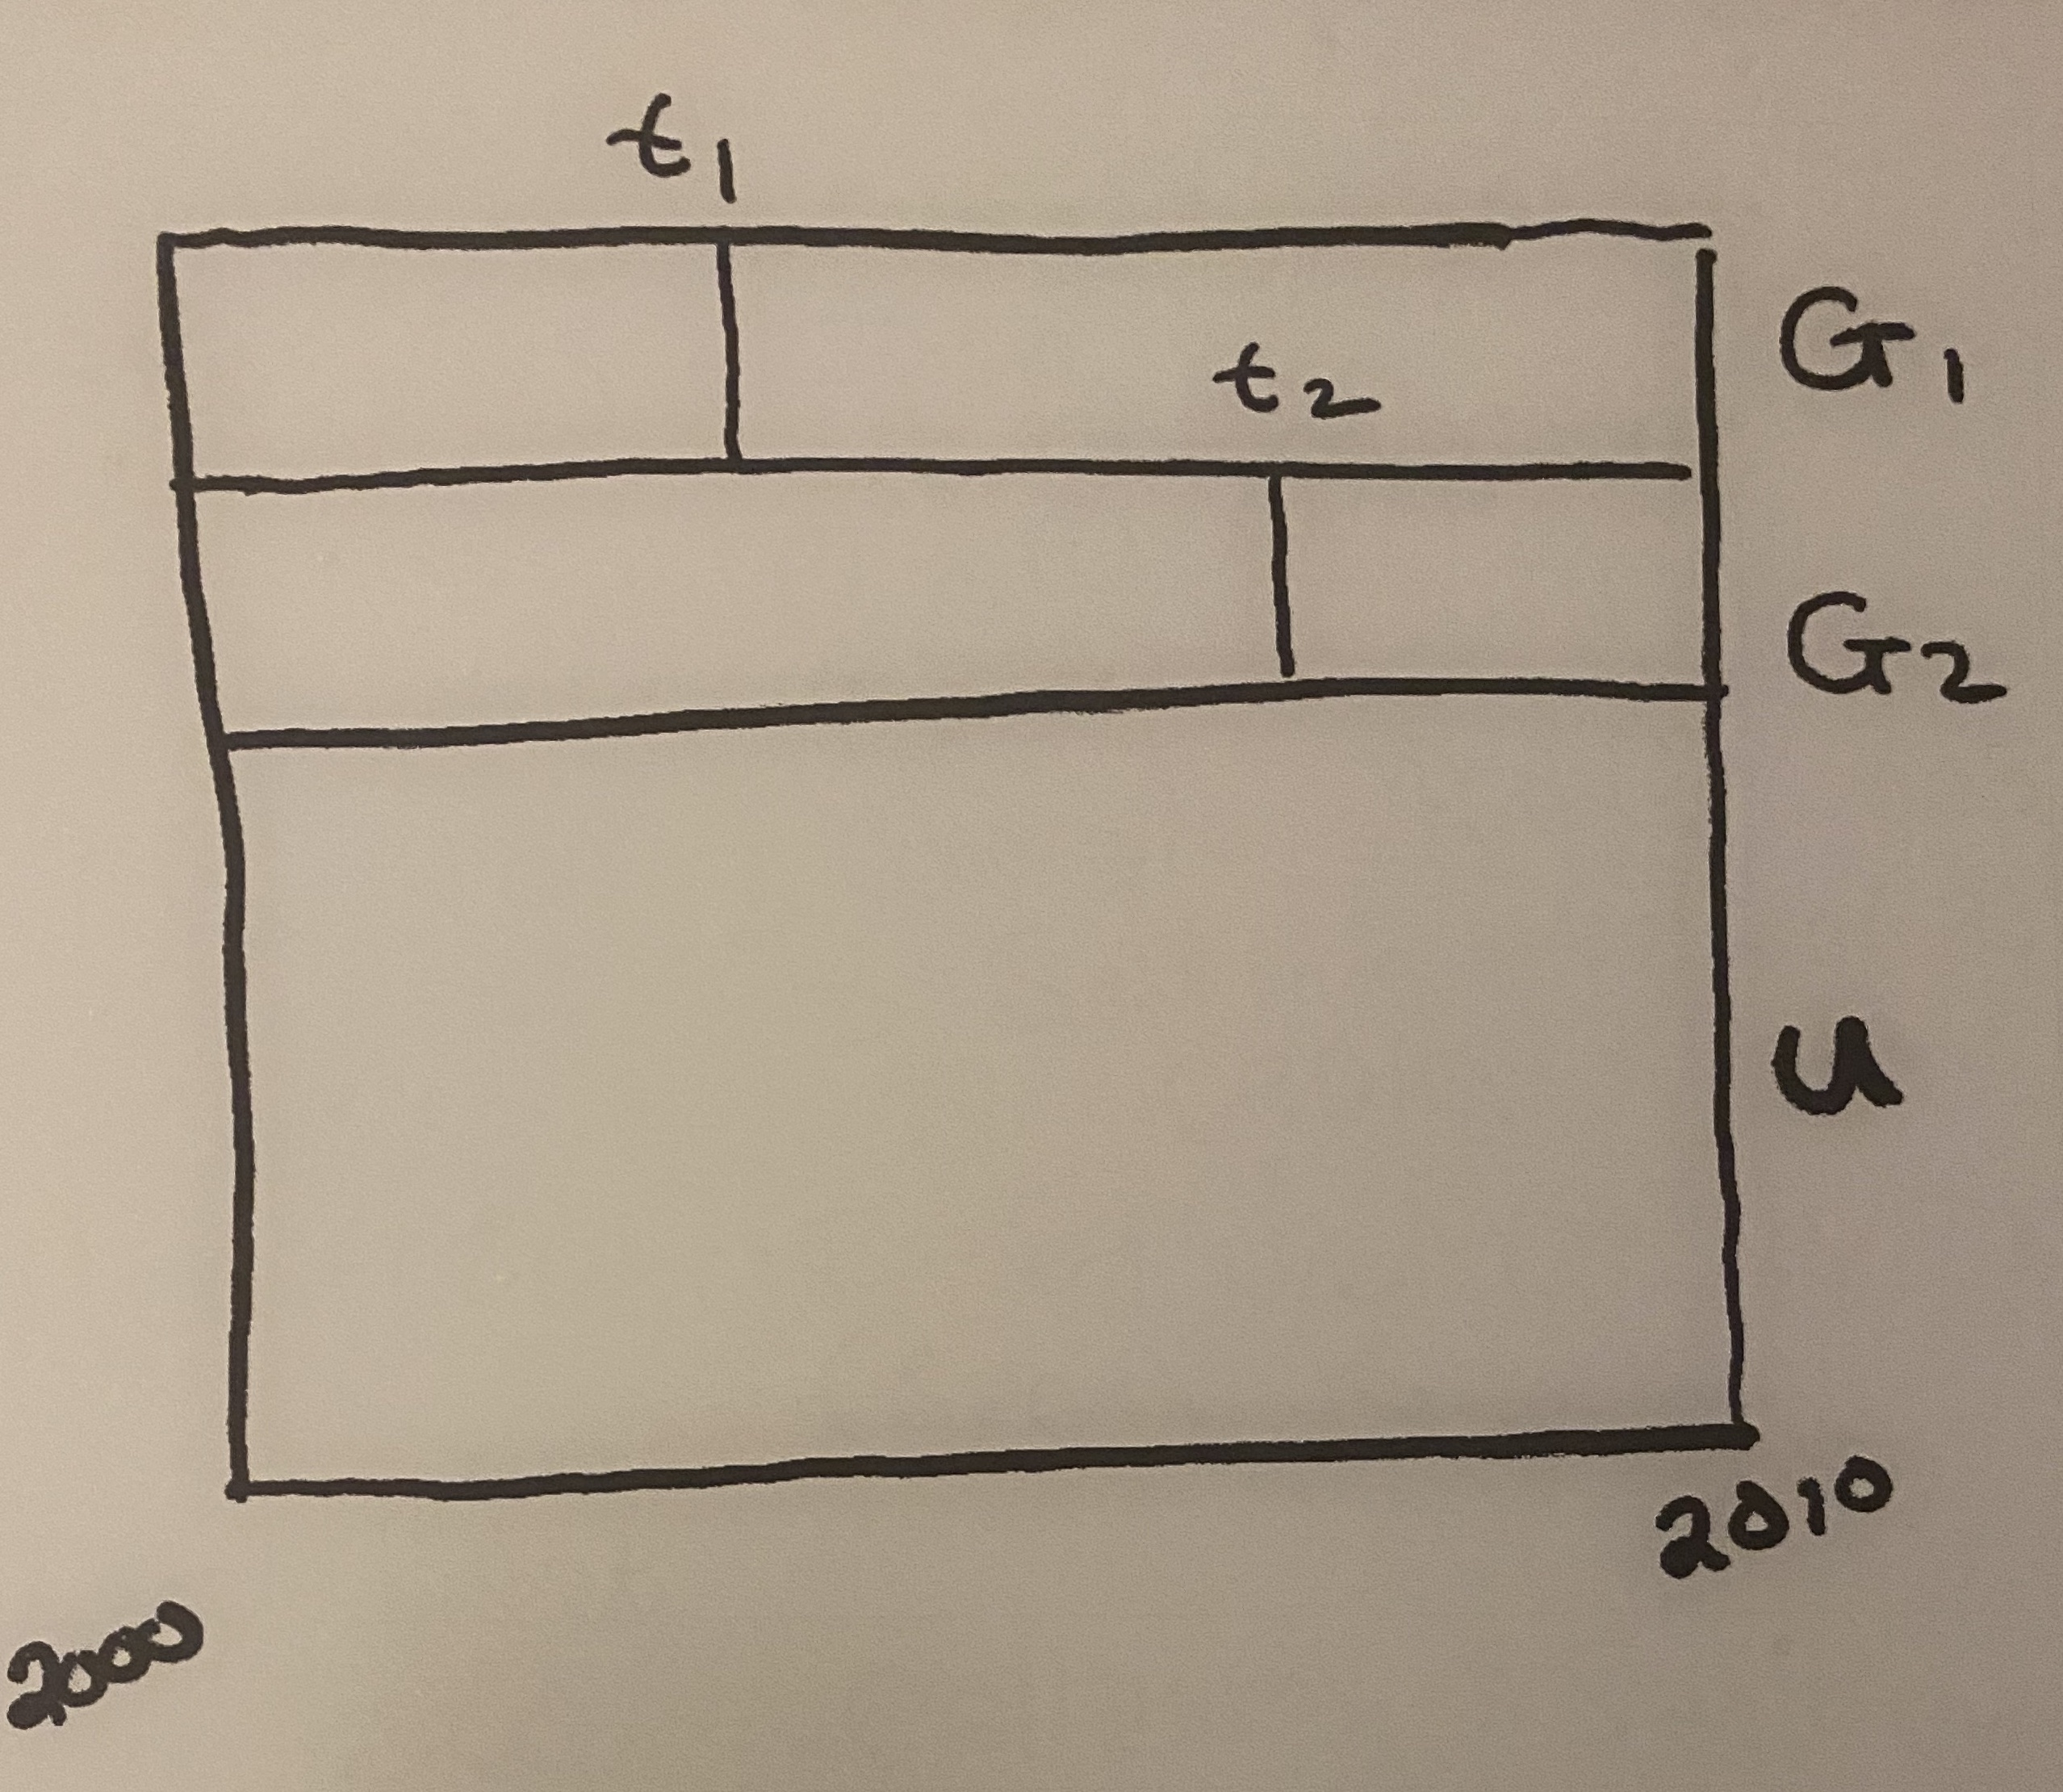
\includegraphics[scale=0.1]{./lecture_includes/stacked1.jpg}
	\end{figure}

\end{frame}


\begin{frame}{Creating $G_1$ dataset: choose max pre (-a) and post (+b) periods}

	\begin{figure}
	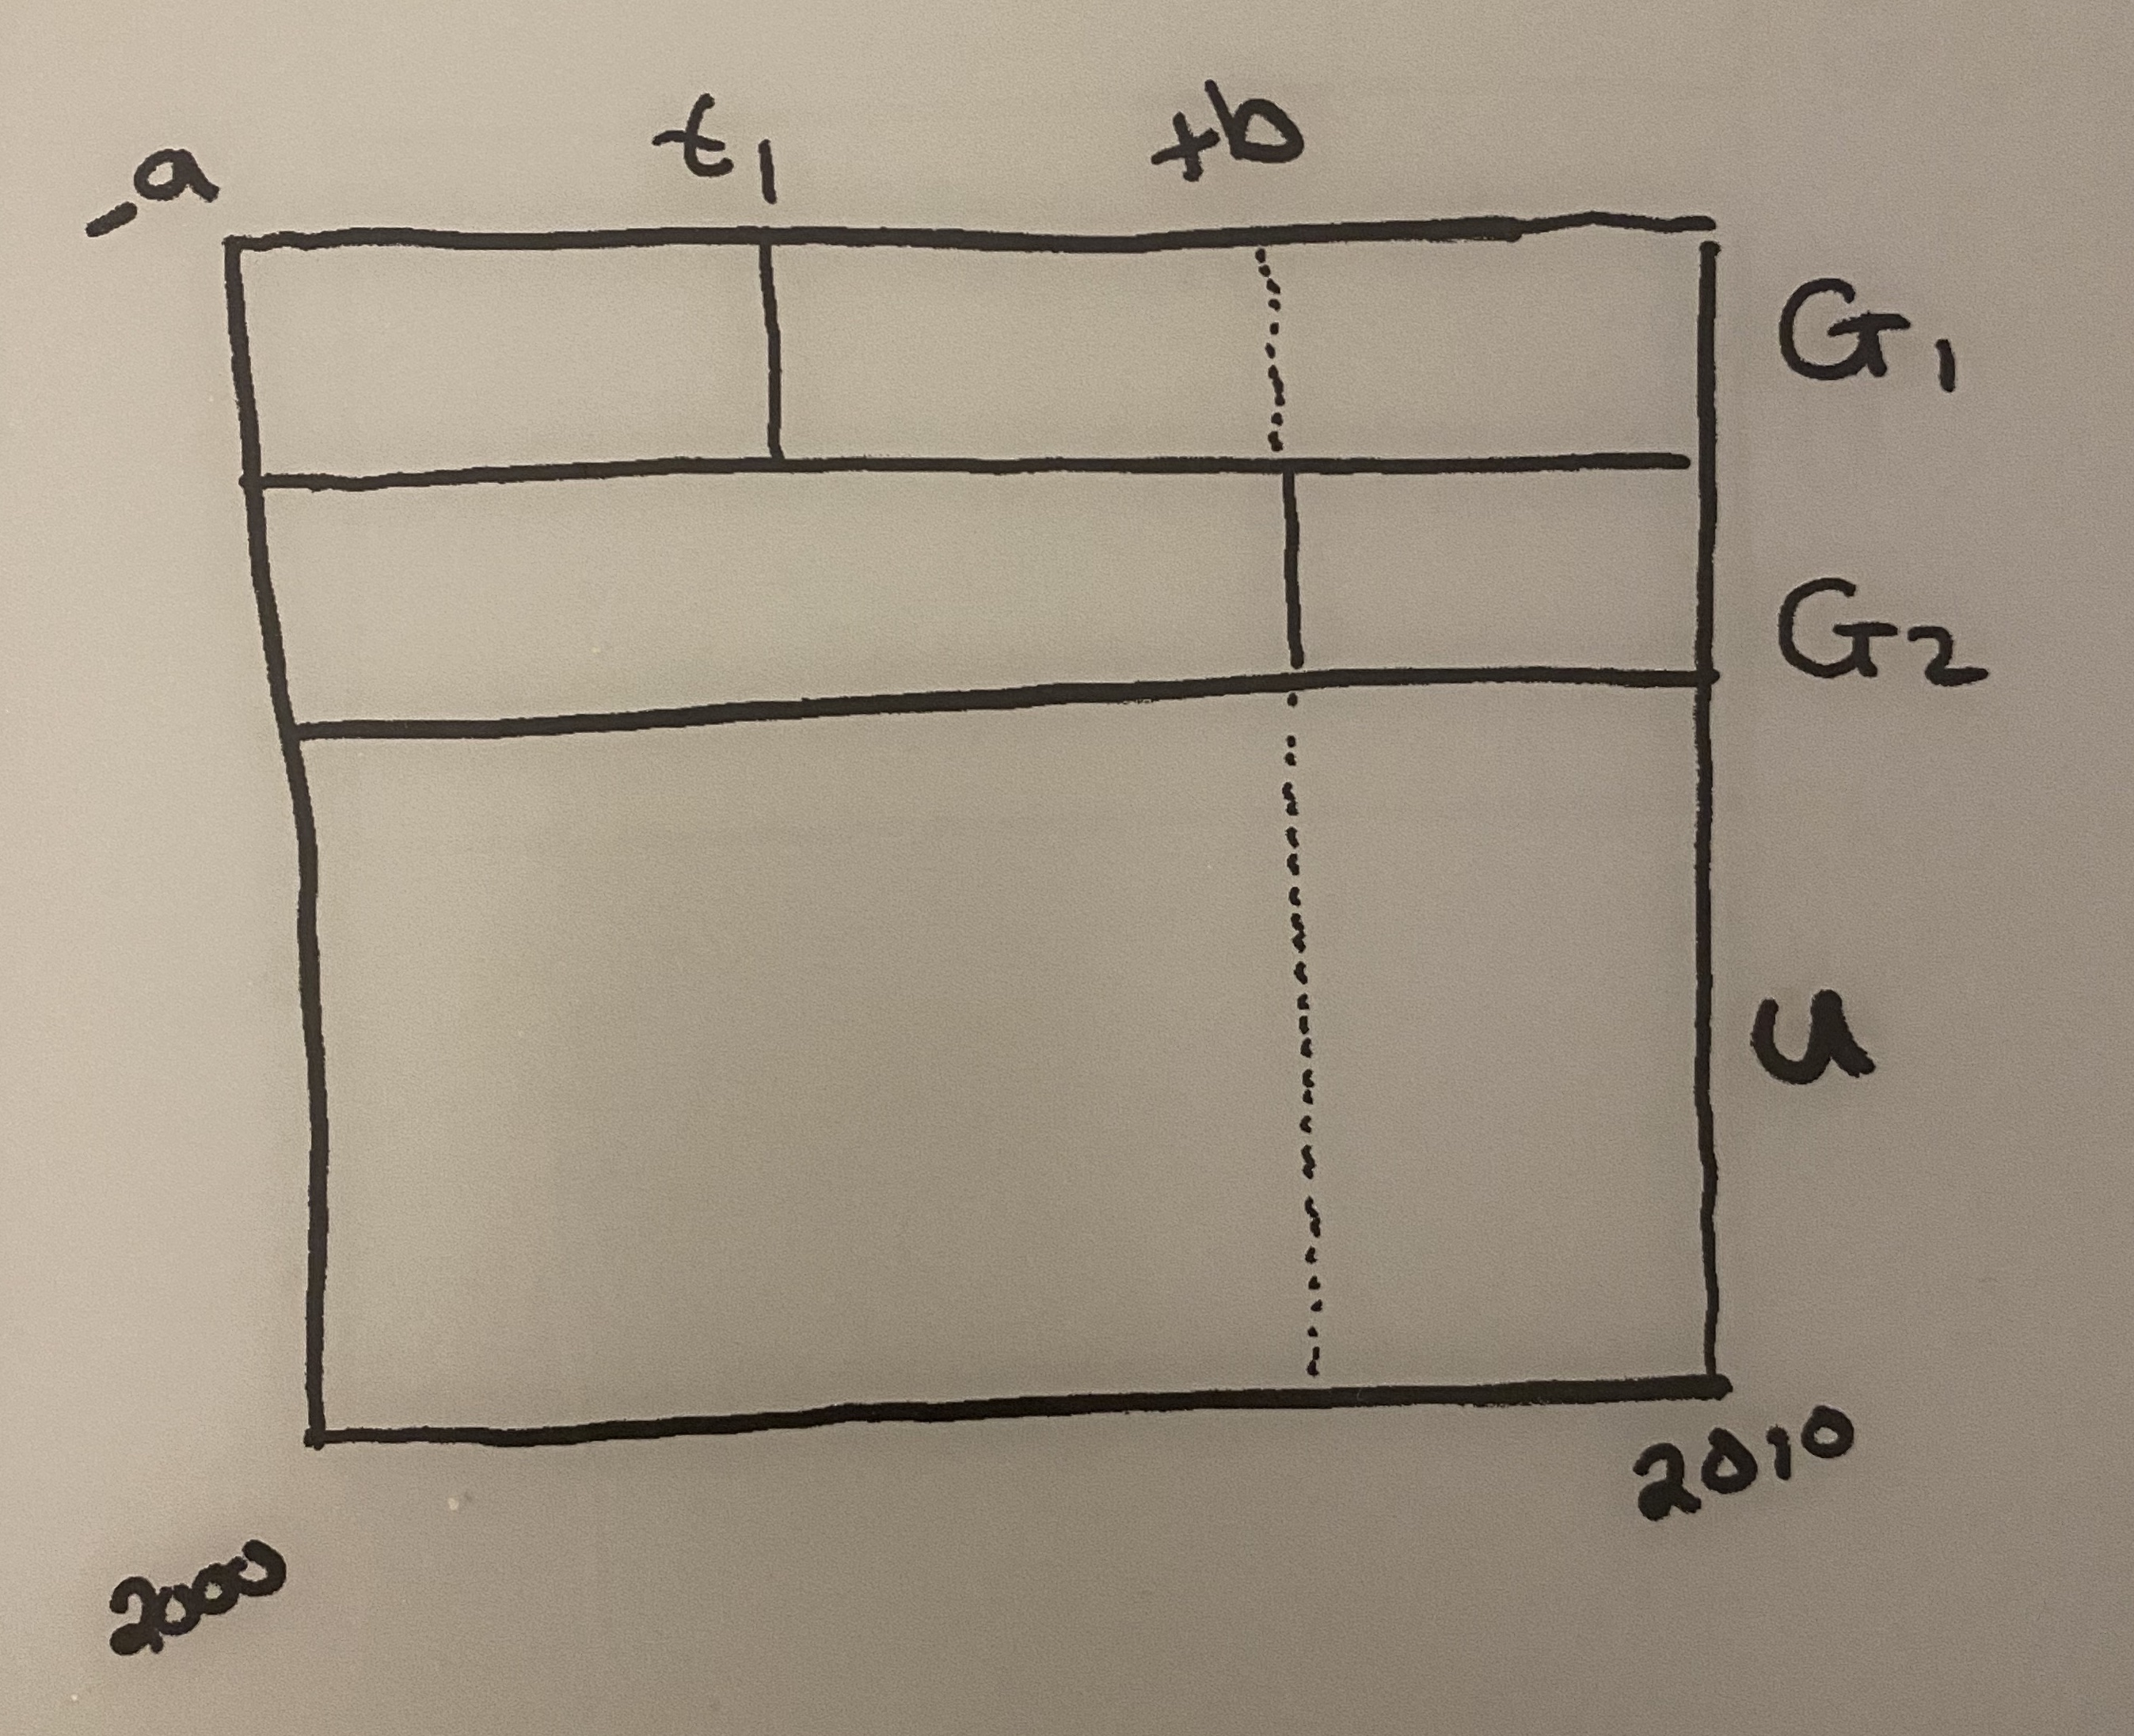
\includegraphics[scale=0.1]{./lecture_includes/stacked2.jpg}
	\end{figure}

\end{frame}

\begin{frame}{Creating $G_1$ dataset: keep untreated units on [-a,+b]}

	\begin{figure}
	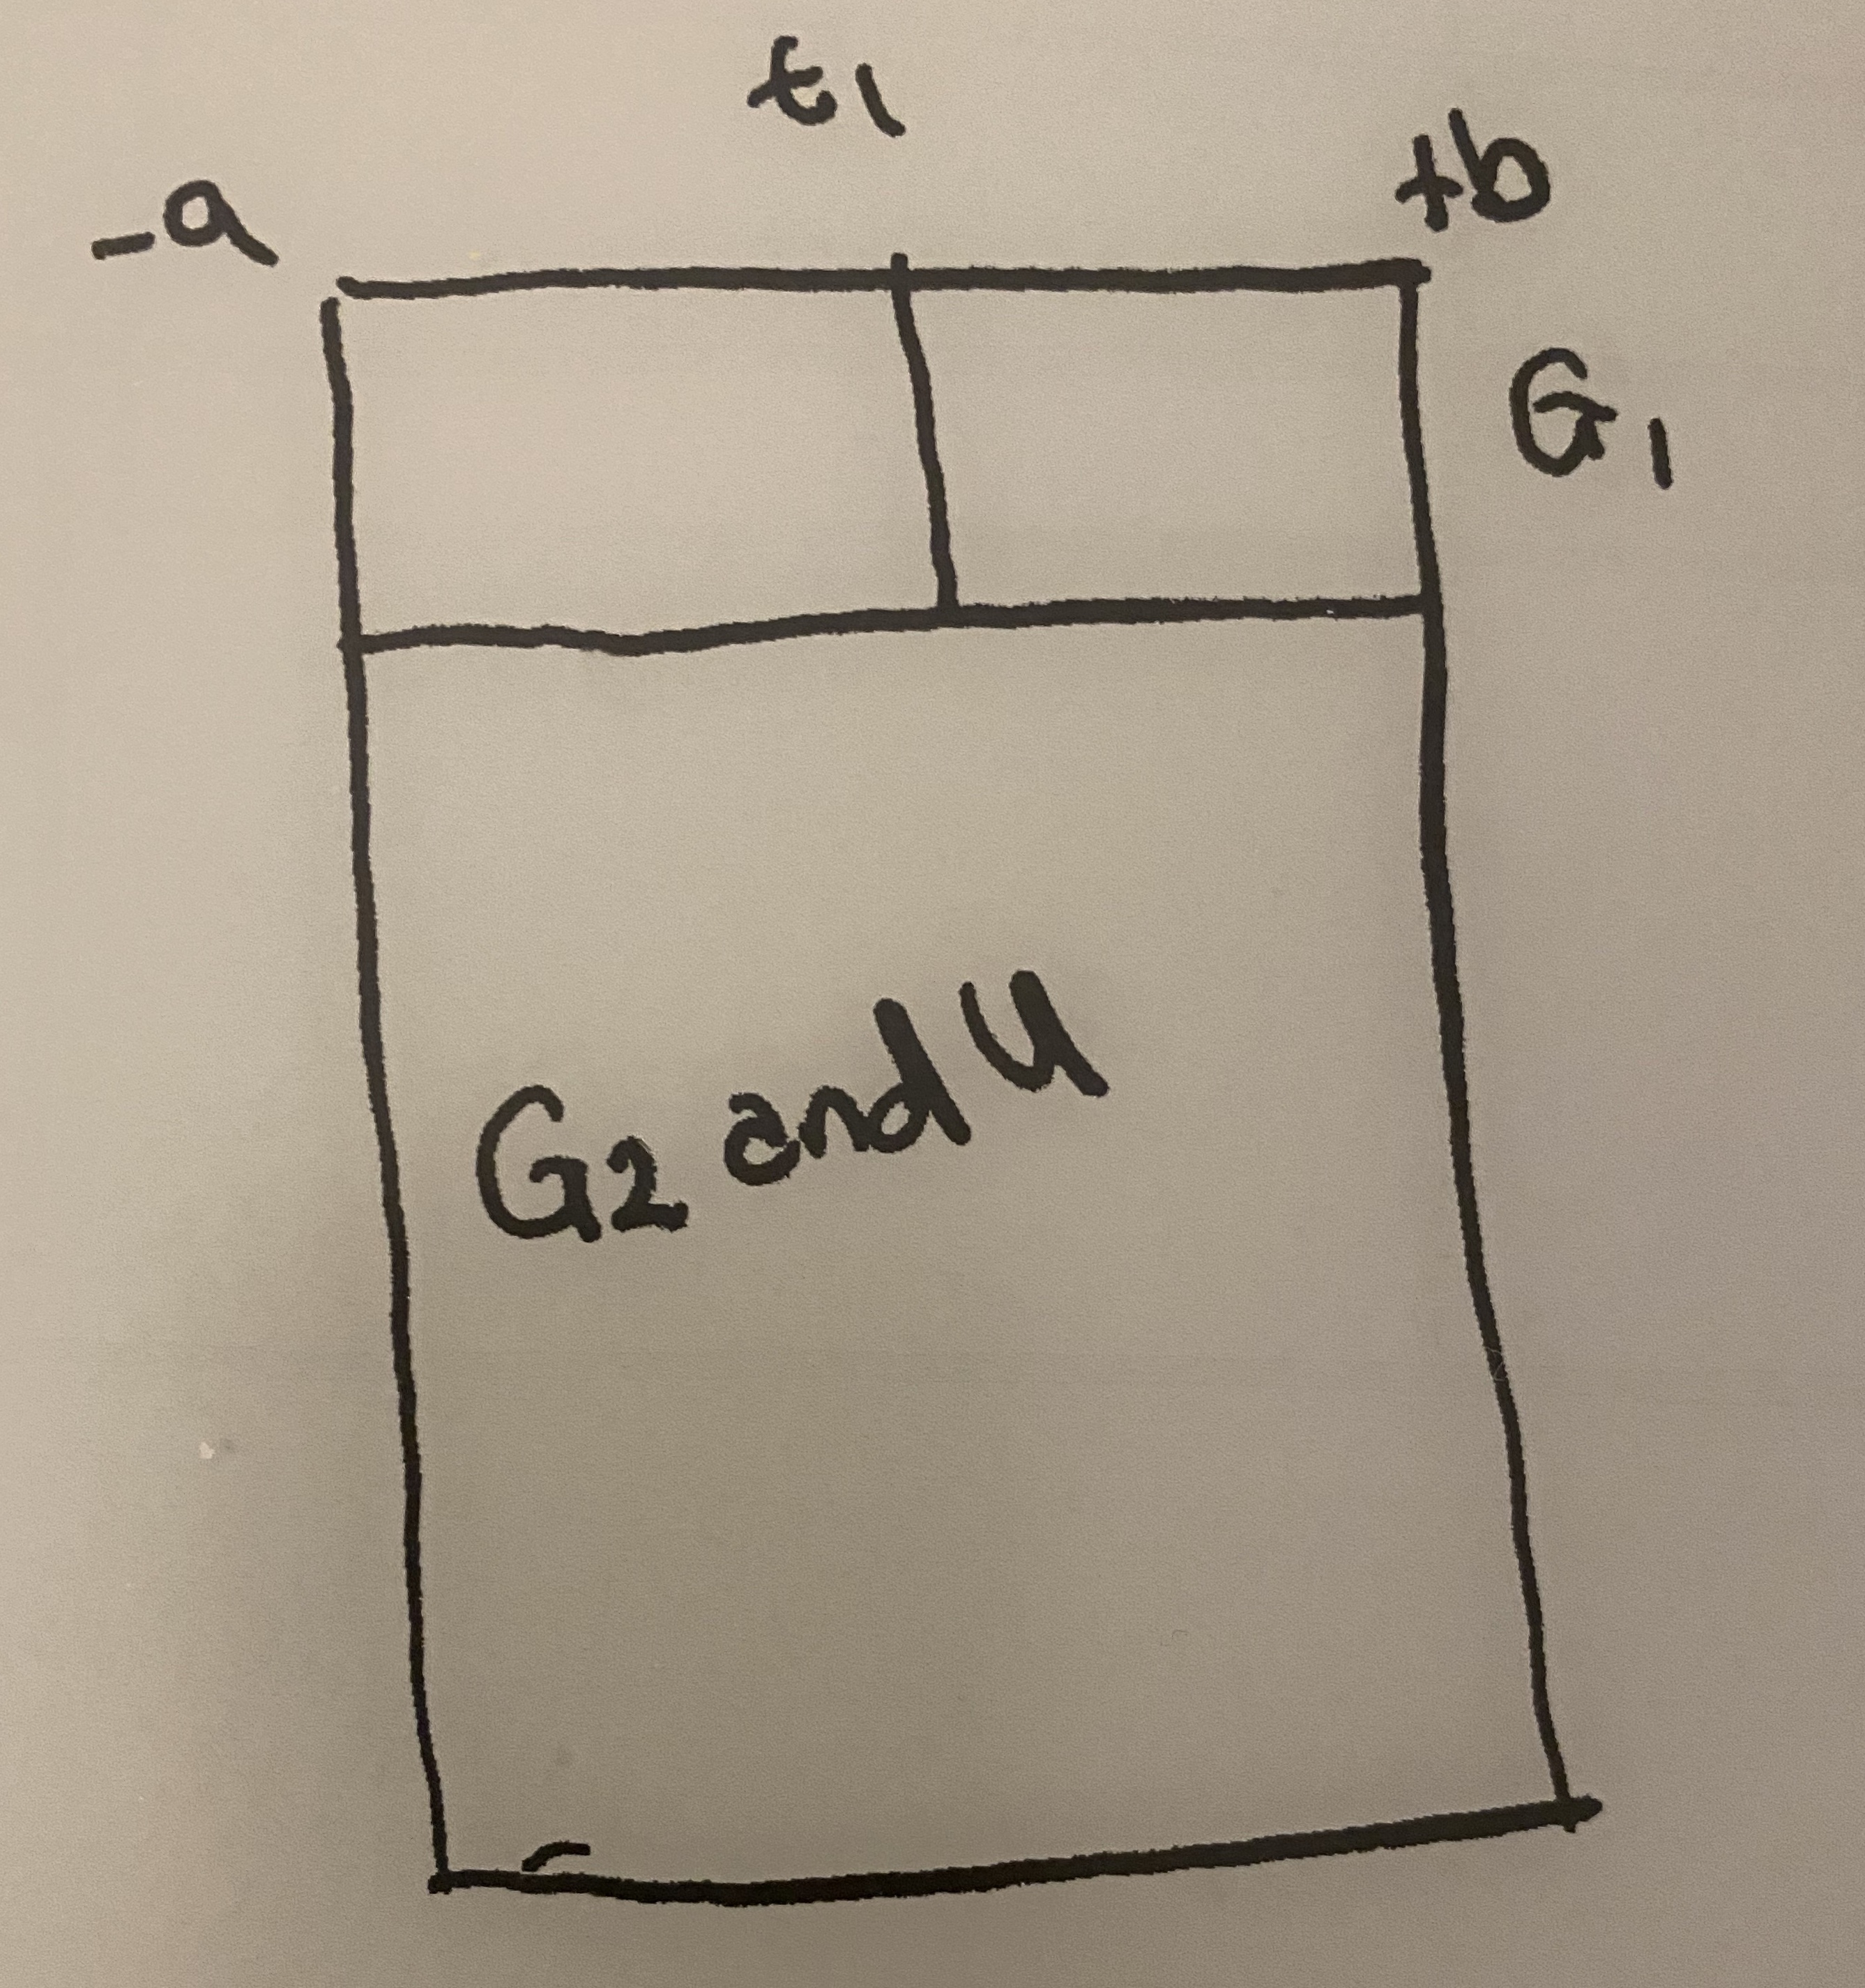
\includegraphics[scale=0.085]{./lecture_includes/stacked3.jpg}
	\end{figure}

\end{frame}


\begin{frame}{Creating $G_2$ dataset: keep \emph{only} untreated units on [-a,+b] intervals as controls}

	\begin{figure}
	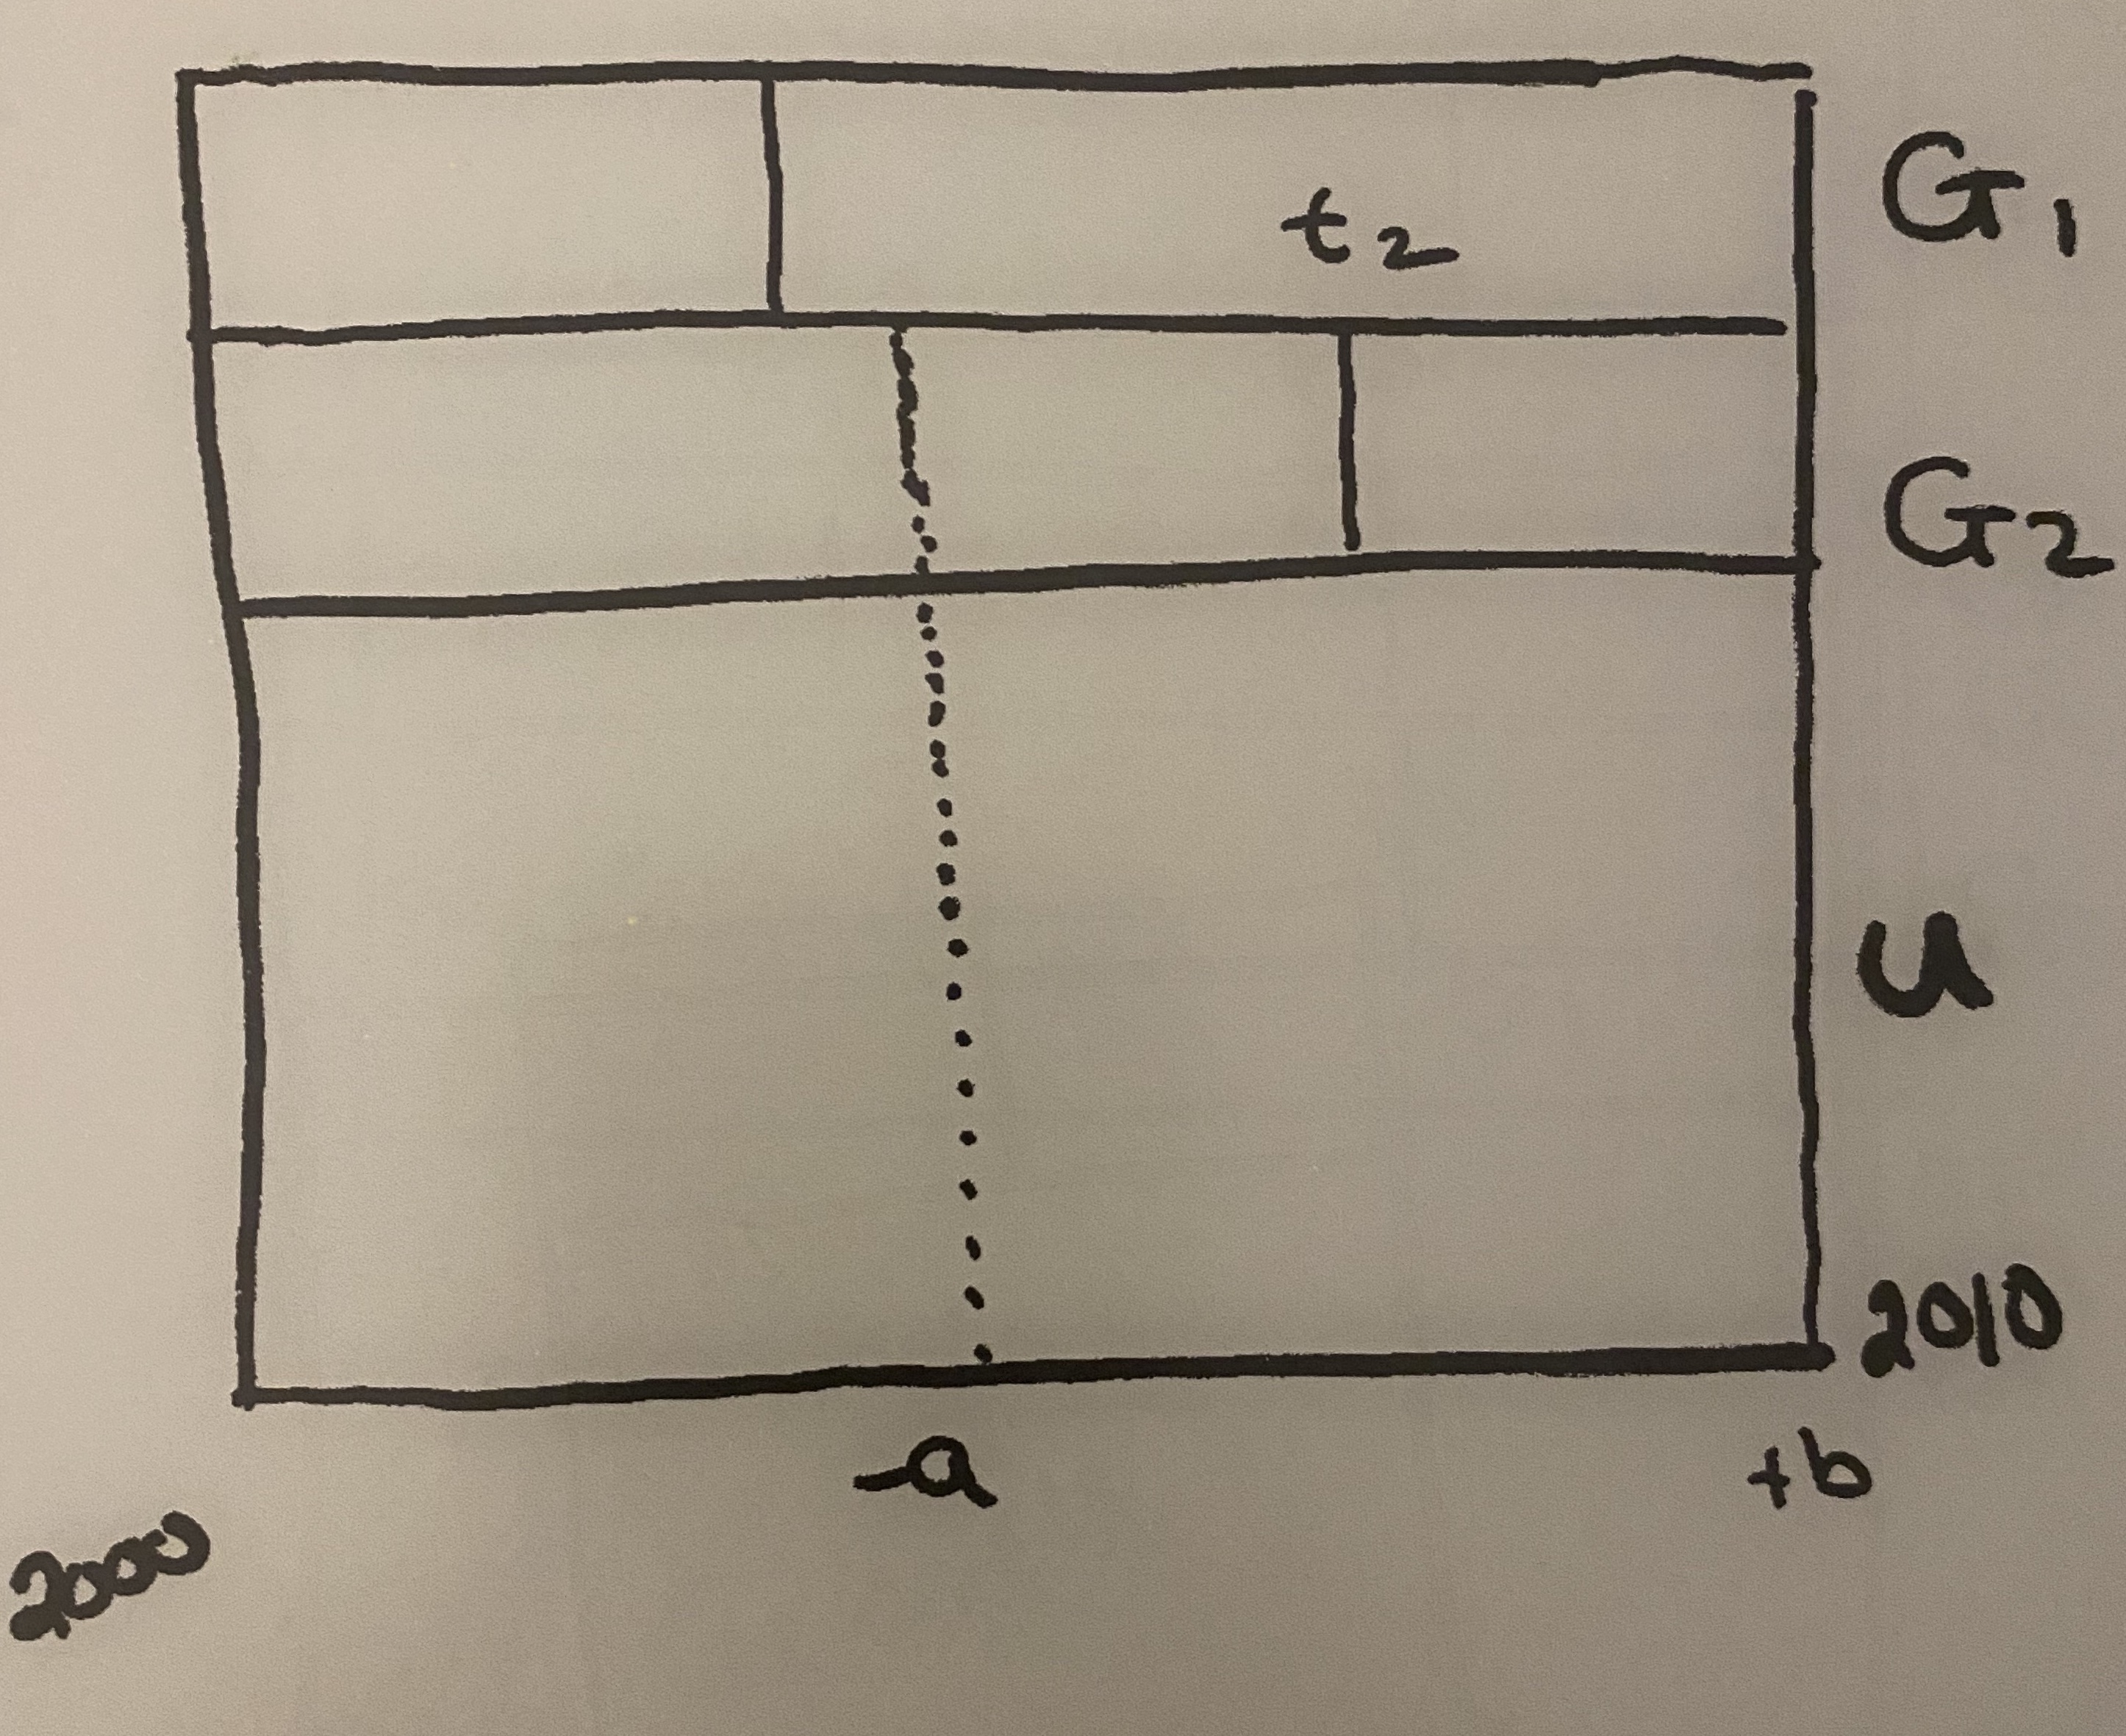
\includegraphics[scale=0.085]{./lecture_includes/stacked4.jpg}
	\end{figure}

\end{frame}


\begin{frame}{Creating $G_2$ dataset: save the dataset}

	\begin{figure}
	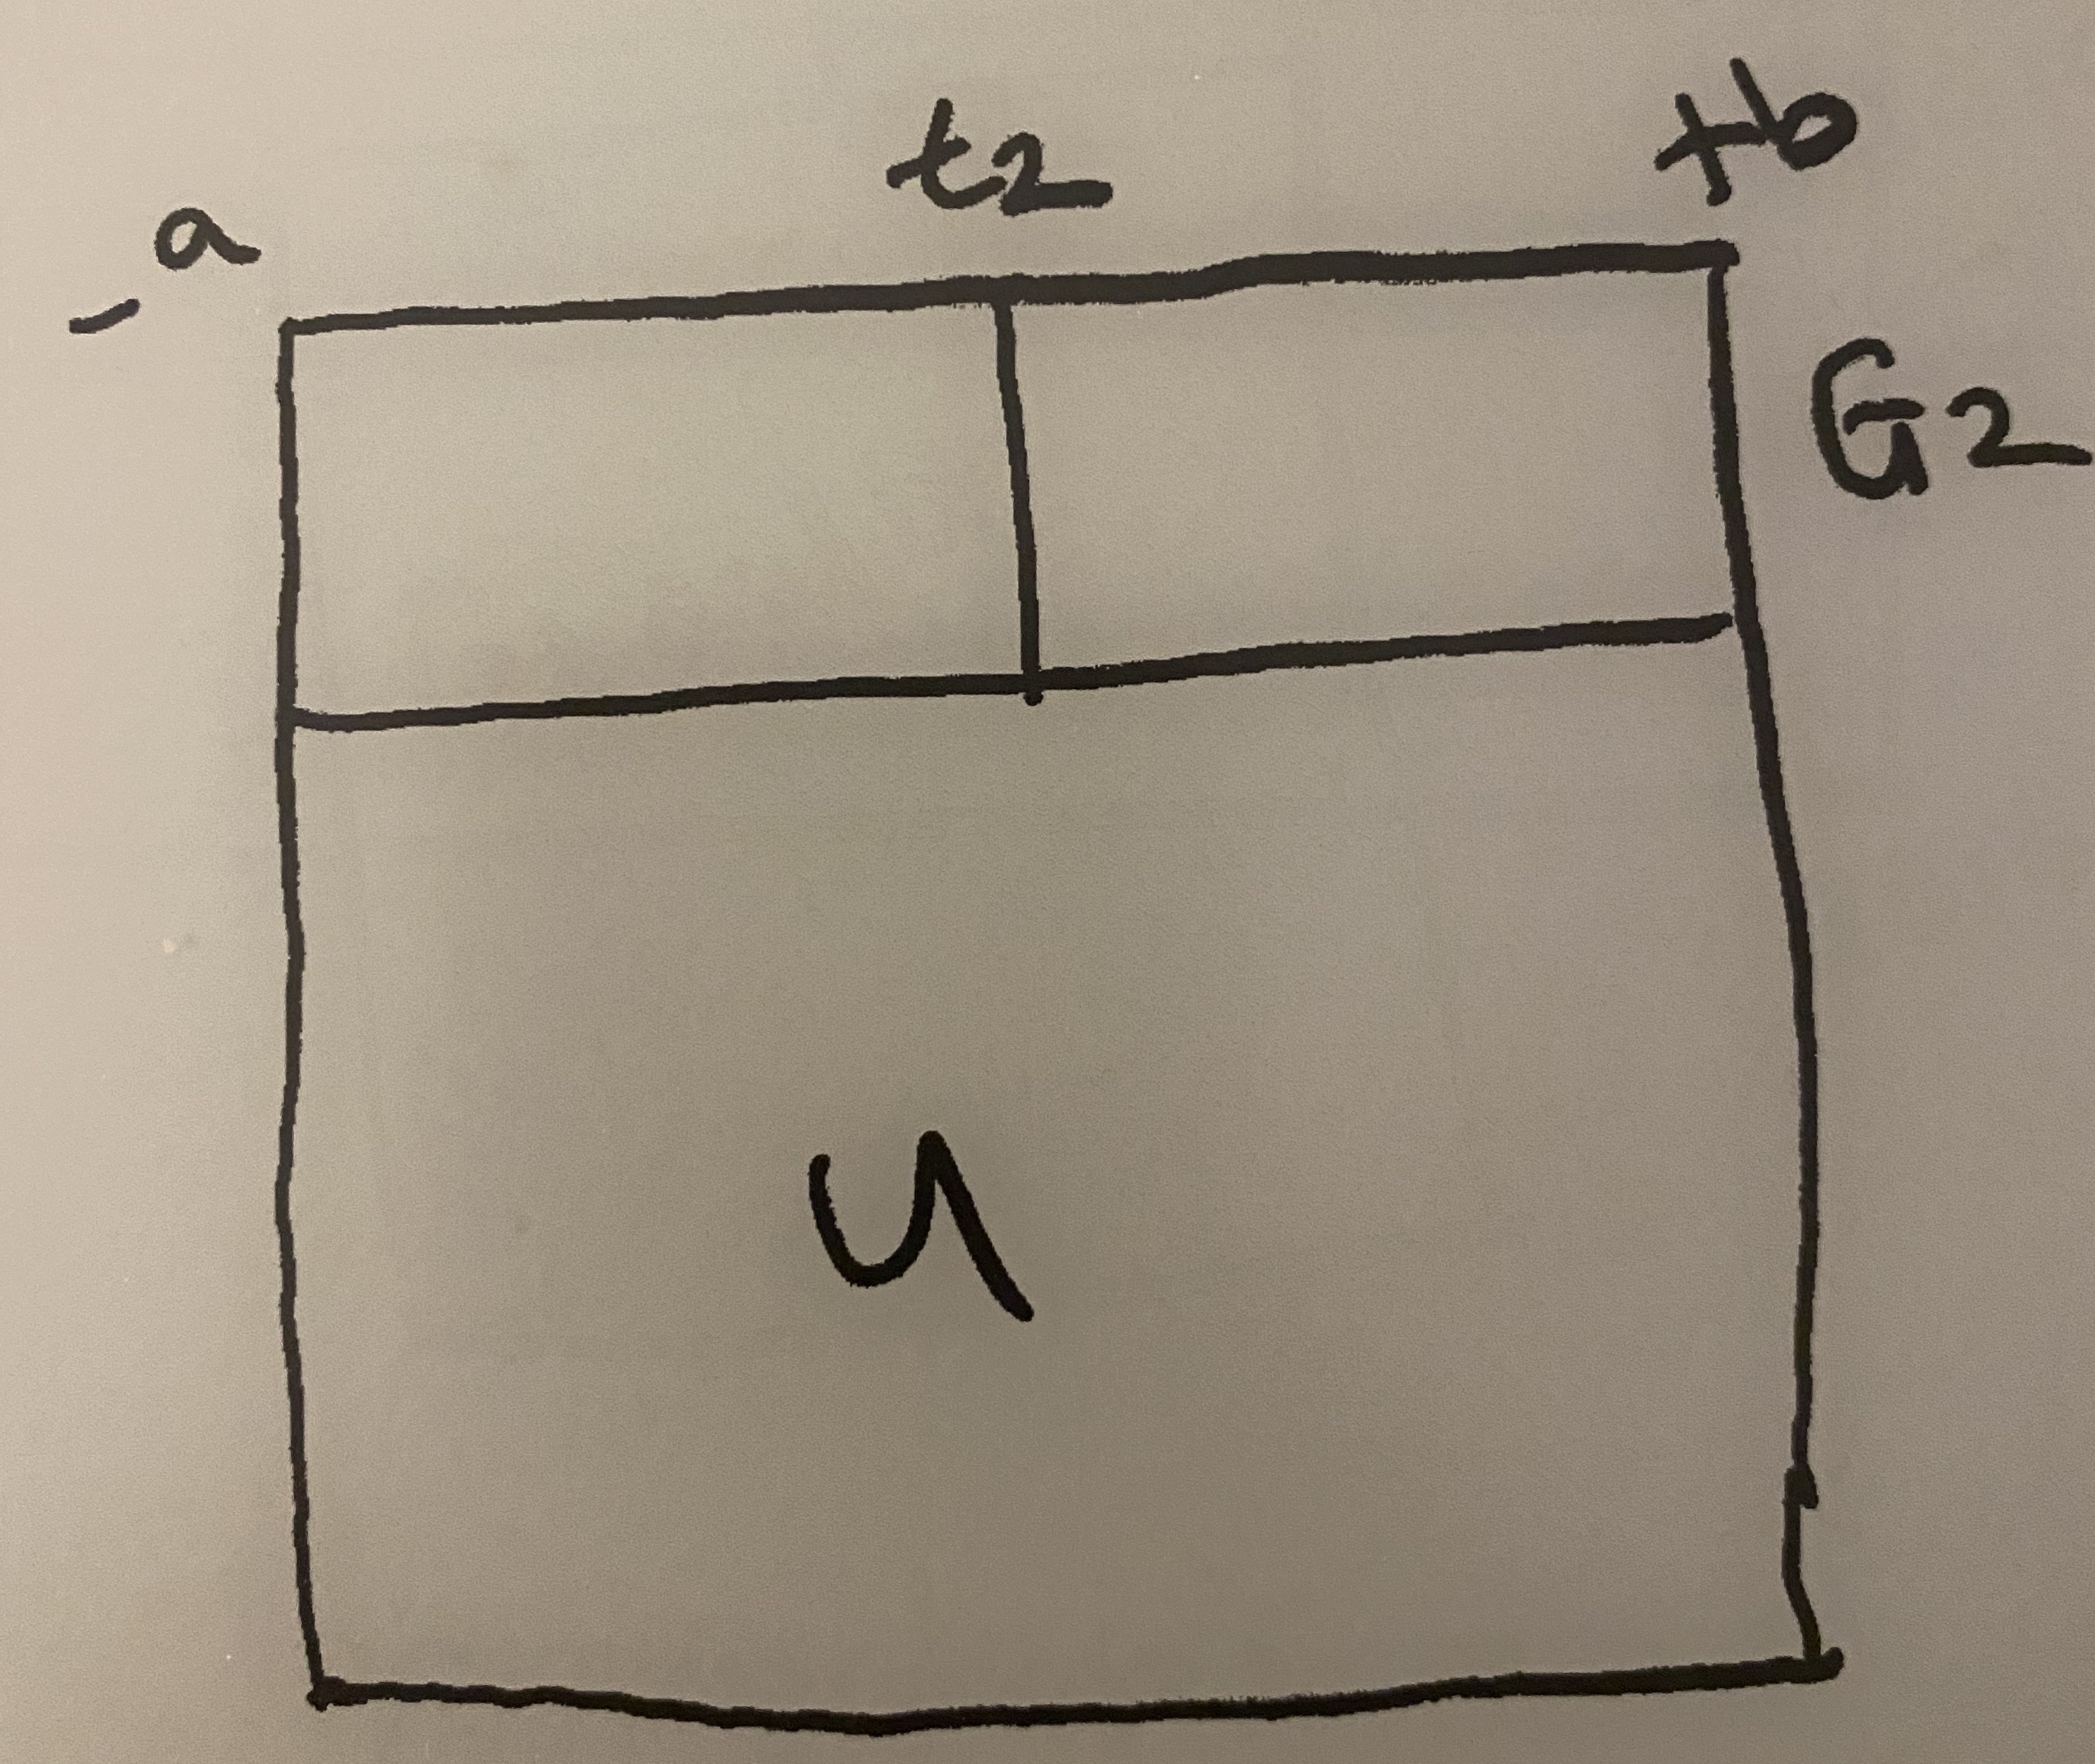
\includegraphics[scale=0.085]{./lecture_includes/stacked5.jpg}
	\end{figure}

\end{frame}


\begin{frame}{Creating $G_2$ dataset: stack the datasets}

	\begin{figure}
	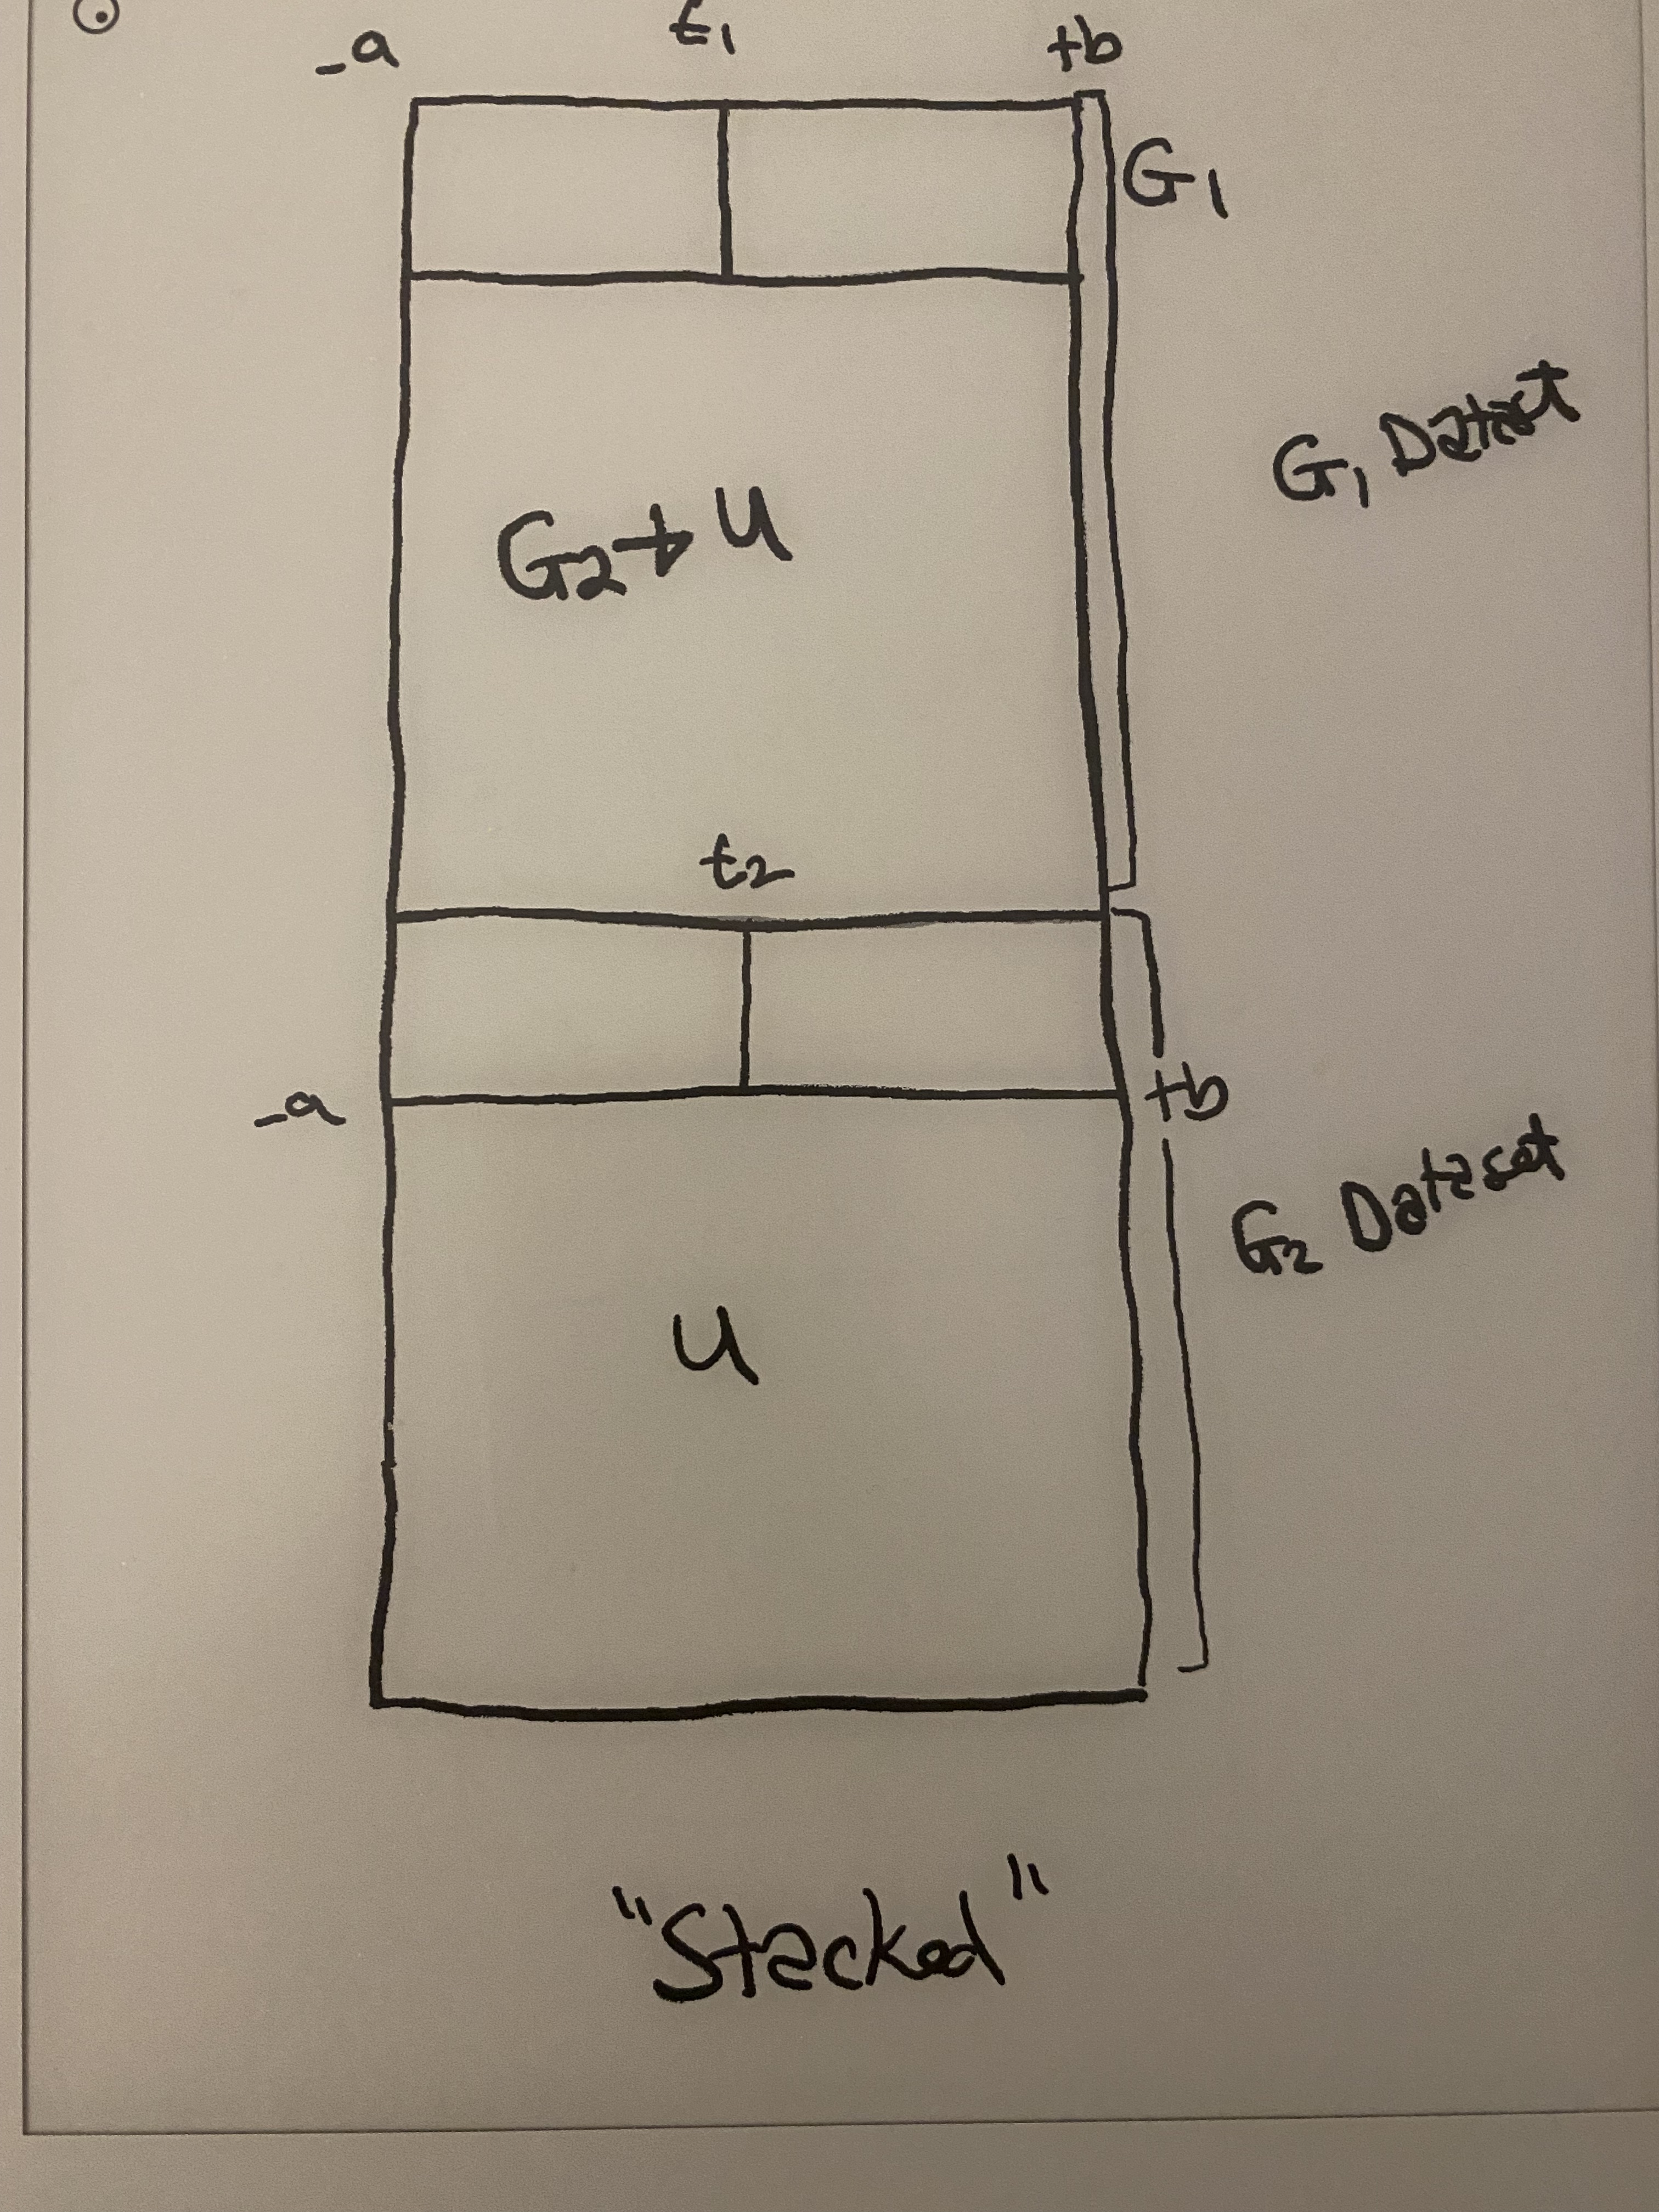
\includegraphics[scale=0.06]{./lecture_includes/stacked6.jpg}
	\end{figure}

\end{frame}



\begin{frame}{Discussion of the stacked data}

\begin{itemize}
\item Why doesn't $G_1$ appear in $G_2$?
\item Notice that $U$ appears in both $G_1$ and $G_2$ datasets. 
\item Unclear to me exactly what Cengiz, et al. (2019) run in their stacked regression, but we probably need to say it now that we want to have a control for ``dataset-by-state'' fixed effects some units appear more than once (e.g., $U$).
\end{itemize}

\end{frame}

\imageframe{./lecture_includes/dube_j.pdf}
\imageframe{./lecture_includes/dube_k.pdf}

\begin{frame}{Upper part of wage distribution}

Logic is used to dismiss effects at upper part of distribution which is only place they find effects

\end{frame}

\imageframe{./lecture_includes/dube_l.pdf}
\imageframe{./lecture_includes/dube_m.pdf}
\imageframe{./lecture_includes/dube_n.pdf}


\subsection{Identification and aggregation}

\subsection{Weights and Parameter}

\begin{frame}{Unknown parameter}

\begin{itemize}
\item Recall CS and SA start with parameter (e.g., group-time ATT) then build the estimator that finds it using aggregation
\item Stacking goes in reverse: start with TWFE using a restructured dataset with ``clean controls''
\item So what is stacking identifying?  VWATT? What are its assumptions?  What are the weights?
\end{itemize}

\end{frame}


\begin{frame}{Identification}

\begin{itemize}
\item Stacking is a TWFE estimation method, except that by balancing in relative event time, there is no longer any differential timing
\item Thus identification requires a weighted parallel trends assumption, but how exactly?
\item The parallel trends is \emph{the same} as what we saw with our group-time representation
\item Parallel is assumed to hold first \emph{within} stacked dataset, not in the final regression model, which shapes the fixed effects we must employ to ensure it
\end{itemize}

\end{frame}

\begin{frame}{Gardner notation}

\begin{equation}
Y_{cgpit} = \lambda_{cg} + \lambda_{cp} + \beta D_{cgph} + \varepsilon_{cgpit}
\end{equation}

\bigskip

$c$ dataset; $g$ group; $p$ period; $i$th member of group $g$; $t$th time period of period $p$

\bigskip

$D_{cgp}$ is an indicator for whether group $g$ is treated during period $p$ of the group-$c$ dataset; $\beta$ is the group-period ATT; $\widehat{\beta}$ is estimate from TWFE

\end{frame}

\begin{frame}{Weighted ATT}

\begin{eqnarray*}
\widehat{\beta} &=& \sum_{g=1}^G \sum_{p=g}^P w_{gp} \beta_{gp} \\
w_{gp} &=& \frac{(1-\pi_c) \pi_c \rho_c}{\overline{P} \sum_{c=1}^G (1-\pi_c) \pi_c \rho_c}
\end{eqnarray*}

{\small
\bigskip

$\pi_c$ is the fraction of units treated in period $p$ and $\rho_c$ is the population share of observations for a given group/period

\bigskip

The stacked estimator positively weights each group's ATT by dataset-specific treatment variance and sample size which slightly overstates the true average bc $\pi$ and $\rho$ are both fractions.

\bigskip

Like Goodman-Bacon (2021), we see that the weights make $\widehat{\beta}$ slightly biased estimate of ATT. 
}

\end{frame}

\subsection{Heterogeneity analysis}




\begin{frame}{Heterogeneity is nevertheless important}

\begin{itemize}
\item When theory predicts that longrun effects of a policy may differ from shortrun effects, then exploring heterogeneity is required
\item Effects may also differ for size of policy which creates problems for SUTVA bc of ``no hidden variation in treatment''
\item But heterogeneity analysis, we said, can introduce p-hacking even subconsiously or due to the ``garden of forking paths'' (Gelman and Loken 2013)
\end{itemize}

\end{frame}


\begin{frame}{P-hacking}

\footnotesize
\begin{quote}
``Here's the thing: P-values of .05 aren't that hard to find if you sort the data differently or perform a huge number of analyses. In flipping coins, you'd think it would be rare to get 10 heads in a row. You might start to suspect the coin is weighted to favor heads and that the result is statistically significant.

\bigskip

But what if you just got 10 heads in a row by chance (it can happen) and then suddenly decided you were done flipping coins? If you kept going, you'd stop believing the coin is weighted.

\bigskip

Stopping an experiment when a p-value of .05 is achieved is an example of p-hacking. But there are other ways to do it -- like collecting data on a large number of outcomes but only reporting the outcomes that achieve statistical significance. By running many analyses, you're bound to find something significant just by chance alone.''

\end{quote}

\end{frame}


\begin{frame}{Alternatives to p-hacking heterogeneity}

\begin{enumerate}
\item \textbf{Preregistration of study designs}: Scientists publicly commit to an experiment's design before the data collection phase or the analysis phase. Much harder to `cherry pick' results
\item \textbf{Open data sharing}: Journals are increasingly requiring that researchers post their data online, or submit to a data repository
\item \textbf{Replication}: Some journals are publishing replications (e.g., Nature's ReScienceX)
\end{enumerate}

\bigskip

Clemens and Strain (2021) use preregistration which is rare in labor or quasi-experimental work but is very common in development economics using RCTs 

\end{frame}

\begin{frame}{Researchers must make choices}

\begin{itemize}
\item Nick Huntington-Klein and several others published a 2021 article in \emph{Economic Inquiry} in which two applied microeconomics papers were assigned to individual researchers with the task of replicating the results from raw data
\begin{quote}
"We find large differences in data preparation and analysis decisions, many of which would not likely be reported in a publication. No two replicators reported the same sample size. Statistical significance varied across replications, and for one of the studies the effect's sign varied as well. The standard deviation of estimates across replications was 3–4 times the mean reported standard error."
\end{quote}
\item Decision making under uncertainty creates variation, not just p-hacking
\end{itemize}

\end{frame}


\begin{frame}{Pre-registration and heterogeneity analysis}

\begin{itemize}
\item Theoretical reasons to suspect effects of the minimum wage may differ depending on whether the bite is large or small
\item Because their analysis would be conducting heterogeneity analysis, and heterogeneity analysis was one of the causes of the replication crisis, they would pre-register
\item Pre-registered design as extensions of their earlier short-run analysis
\end{itemize}

\end{frame}




\begin{frame}{Variation in treatment}


\begin{quote}
``Consider an assessment of the causal effect of aspirin on headaches. For the potential outcome with both of us taking aspirin, we obviously need more than one aspirin tablet.  Suppose, however, that one of the tablets is old and no longer contains a fully effective dose, whereas the other is new and at full strength.  In that case, each of us may have three treatments available: no aspirin, the ineffective tablet, and the effective tablet.  There are thus two forms of the active treatment, both nominally labeled ``aspirin'': aspirin+ and aspirin-.'' (Imbens and Rubin 2015)
\end{quote}

\end{frame}


\begin{frame}{SUTVA}	

Stable Unit Treatment Value Assumption requires that an individual receiving a specific treatment level cannot receive different forms of that treatment (called the ``no hidden variations of treatments'' by Imbens and Rubin 2015)

\bigskip

\begin{quote}
``One strategy to make SUTVA more plausible relies on redefining the represented treatment levels to comprise a larger set of treatments, for example, Aspirin-, Aspirin+ and no-aspirin instead of only Aspirin and no-aspirin.'' (Imbens and Rubin 2015)
\end{quote}

\end{frame}


\begin{frame}{Great Recession}

\begin{itemize}
\item Great Recession saw a pause in minimum wage hikes followed by large increases in several states
\item Increases in Cengiz, et al. (2019) were around 8 log points on average; minimum wage increases after the Great Recession range from 25 log points to as high as 60 log points (Clemens and Strain 2021)
\item ``DC, CA and NY had increased their minimum wages by 61, 50 and 53 percent respectively.''
\end{itemize}

\end{frame}



\begin{frame}{Methodology and Data}

\begin{itemize}
\item Data: American Community Survey and Current Population Survey: 
	\begin{itemize}
	\item Years: 2011-2015 with pre-registration commitment to study through 2019
	\end{itemize}
\item Methodologies:
	\begin{itemize}
	\item TWFE event study
	\item Stacked regression (Cengiz, et al. 2019; Baker, et al. 2020)
	\item Imputation estimator (Borusyak, Jaravel and Spiess 2021)
	\end{itemize}
\item Unique characteristics of treatment: large and small increases will be modeled separately
\end{itemize}

\end{frame}


\begin{frame}{Summary of findings}

\begin{itemize}
\item Large increases in minimum wages reduced employment rates among individuals with low levels of experience and education by just over 2.5pp
\item Relatively small minimum wage increases are variable and centered on zero much like what Cengiz, et al. (2019) found
\item Medium-run effects are larger and more negative than short-run effects
\end{itemize}

\end{frame}

\begin{frame}[shrink=20]{TWFE Event study specification}

\begin{eqnarray*}
Y_{i,s,g(s),t} = \sum_{g(s) \neq 0} \beta_{g(s)}Policy_{g(s)} \times Post_t + \alpha_{1s} State_s + \alpha_{2t} Time_t + X_{i,s,t} \gamma + \varepsilon_{i,s,t}
\end{eqnarray*}

\bigskip

$Y$ is binary for employment for person $i$ in state $s$ in policy category $g(s)$ and time $t$.  Samples are restricted to young (16-21yo) without high school, and young overall (16-25yo).  $X$ are the ``rich controls'' they label later and it includes median house price index, log aggregate personal income per capita, employment rates for different skill levels, and individual-level demographic controls.  

\bigskip

Coefficients of interest are the $\beta$ terms and 2014 will be treated as the transition year.  It measures the causal effect of state minimum wage policy changes on employment under standard, albeit nontrivial, assumptions such as homogenous treatment effects over time, no anticipation and parallel trends. 

\bigskip

They will also estimate triple difference versions of this model with a within-state control group of untreated workers.


\end{frame}


\imageframe{./lecture_includes/Clemens_twfe_2.png}
\imageframe{./lecture_includes/Clemens_twfe_1.png}
\imageframe{./lecture_includes/Clemens_twfe_3.png}


\begin{frame}{Extension 1: Stacked regression}

\begin{itemize}
\item Remember the big idea: create a new, much larger, dataset by appending the same dataset to itself over and over, not in balanced calendar time, but in balanced \emph{event time}.
\item Then estimate a simple TWFE model controlling for dataset-by-state fixed effects
\end{itemize}

\end{frame}

\imageframe{./lecture_includes/Clemens_stacked_1.png}


\begin{frame}{Briefly concluding remarks}

\begin{itemize}
\item To understand the rest of their results, we have to first cover the imputation estimator that Borusyak, Jaravel and Speiss (2021) have created
\item But to summarize what we found so far, large shocks are indeed credibly causing declines in employment, particular for the affected class of workers (young with or without a high school degree)
\item More modest increase are null, though, which is what Cengiz, et al. (2019) also found
\item Debates continue!  See my podcast interview with Meer and West, as well as Alan Manning
\end{itemize}

\end{frame}




\end{document}
